% arara: pdflatex
% !arara: indent: {overwrite: yes}
\documentclass[handout]{beamer}
\usepackage[latin1]{inputenc}
\usetheme{Boadilla}
\usecolortheme{seagull}
\usepackage{standalone}
\usepackage{tikz}
\usetikzlibrary{positioning}
\usetikzlibrary{mindmap}
\usetikzlibrary{decorations.text}

\tikzset{
	invisible/.style={opacity=0},
	visible on/.style={alt=#1{}{invisible}},
	alt/.code args={<#1>#2#3}{%
		\alt<#1>{\pgfkeysalso{#2}}{\pgfkeysalso{#3}} % \pgfkeysalso doesn't change the path
	},
}

\title[WeBWorK]{WeBWorK-- a Faculty-driven Homework Management System}
\author[Jordan, Hughes, Yao]{Alex Jordan \and Chris Hughes \and Xialong Yao}
\institute[PCC]{Portland Community College}
\date{February 17, 2014}
\begin{document}

\begin{frame}
	\tikz [remember picture,overlay]
	\node[opacity=0.1] at
	%([yshift=3cm]current page.south)
	(current page.center)
	{\includegraphics[width=.75\textwidth]{WeBWorK-logo-tikz}};
	\titlepage
\end{frame}

%Let me know if there is anything out of place or something you think should be moved to another page.

\begin{frame}
	\centering
	\resizebox{.87\textwidth}{!}{%
		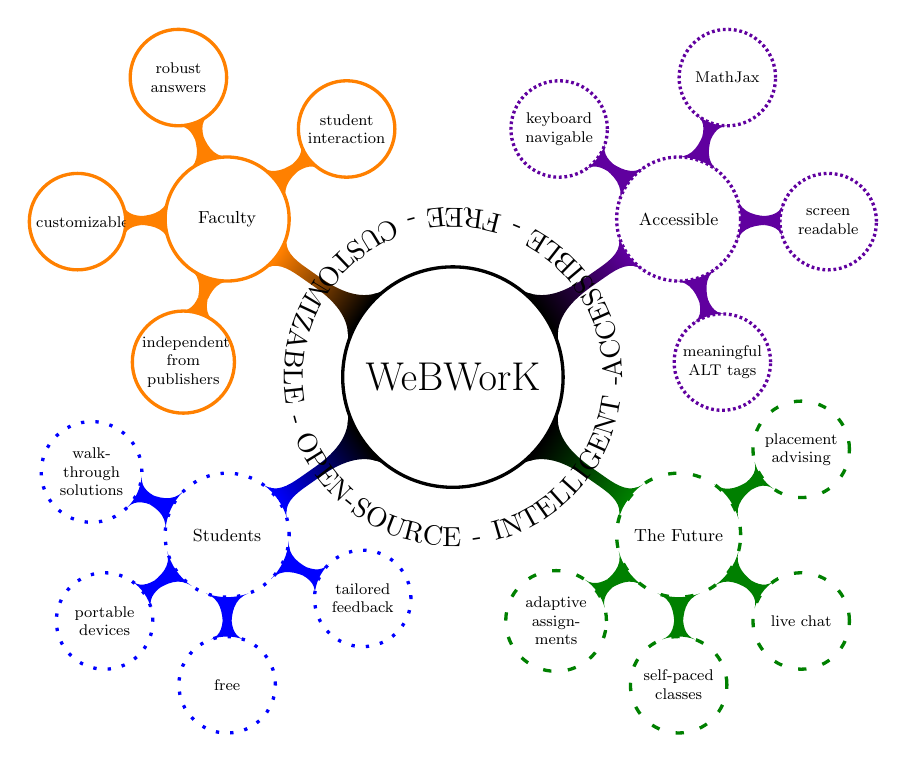
\begin{tikzpicture}[mindmap,
				concept/.append style={fill={none}},
				root concept/.style={concept color=blue},
				level 1 concept/.append style=
				{level distance = 35mm},
				level 2 concept/.append style=
				{level distance = 19mm},
				every node/.append style={align=center,scale=0.7},
			]
			\node [concept,font=\huge] {WeBWorK}
			child[grow=145, concept color=orange,visible on=<2->] {node[concept] {Faculty}
				child[grow=37, visible on=<2->]{node[concept] {student interaction}}
				child[grow=109, visible on=<2->]{node[concept] {robust\\ answers}}
				child[grow=181, visible on=<2->]{node[concept] {customizable}}
				child[grow=253, visible on=<2->]{node[concept] {independent from publishers}}
			}
			child[loosely dotted,concept color=blue,grow=215,visible on=<3->] {node[concept] {Students}
				child[grow=155,visible on=<3->]{node[concept] {walk-through solutions}}
				child[grow=215,visible on=<3->]{node[concept] {portable\\devices}}
				child[grow=270,visible on=<3->]{node[concept] {free}}
				child[grow=335,visible on=<3->]{node[concept] {tailored feedback}}
			}
			child[dash pattern=on 1pt off 1pt on 1pt off 1pt, concept color=blue!50!purple,grow=35,visible on=<4->] {node[concept] {Accessible}
				child[grow=143,visible on=<4-> ] {node[concept] {keyboard navigable}}
				child[grow=71,visible on=<4->] {node[concept] {MathJax}}
				child[grow=359,visible on=<4->] {node[concept]{screen\\ readable} }
				child[grow=287,visible on=<4->] {node[concept] {meaningful ALT tags}}
			}
			child[loosely dashed,concept color=green!50!black,grow=325,visible on=<5->] {node[concept] {The Future}
				child[grow=215,visible on=<4-> ] {node[concept] {adaptive assignments}}
				child[grow=35,visible on=<4->] {node[concept] {placement advising}}
				child[grow=270,visible on=<4->] {node[concept] {self-paced classes}}
				child[grow=-35,visible on=<4->] {node[concept] {live chat}}
			};
			\node at (0,0) [inner sep=15mm,decorate,circle,decoration=
				{raise=10pt,text along path,text={ACCESSIBLE - FREE - CUSTOMIZABLE - OPEN-SOURCE -  INTELLIGENT - },
					text align=fit to path,
				}] {};
		\end{tikzpicture}
	}
\end{frame}

%----------------------------------------------------------------------------------------------------------------------------------------------------------------
\begin{frame}
	timeline- fancy home-made graphic detailing the journey
\end{frame}
\end{document}
